\documentclass[xcolor=dvipsnames]{beamer}
\usepackage{subfig}
\usetheme{Rochester}  %% Themenwahl
\usecolortheme[named=RoyalBlue]{structure}
\usebackgroundtemplate{
	\centering
	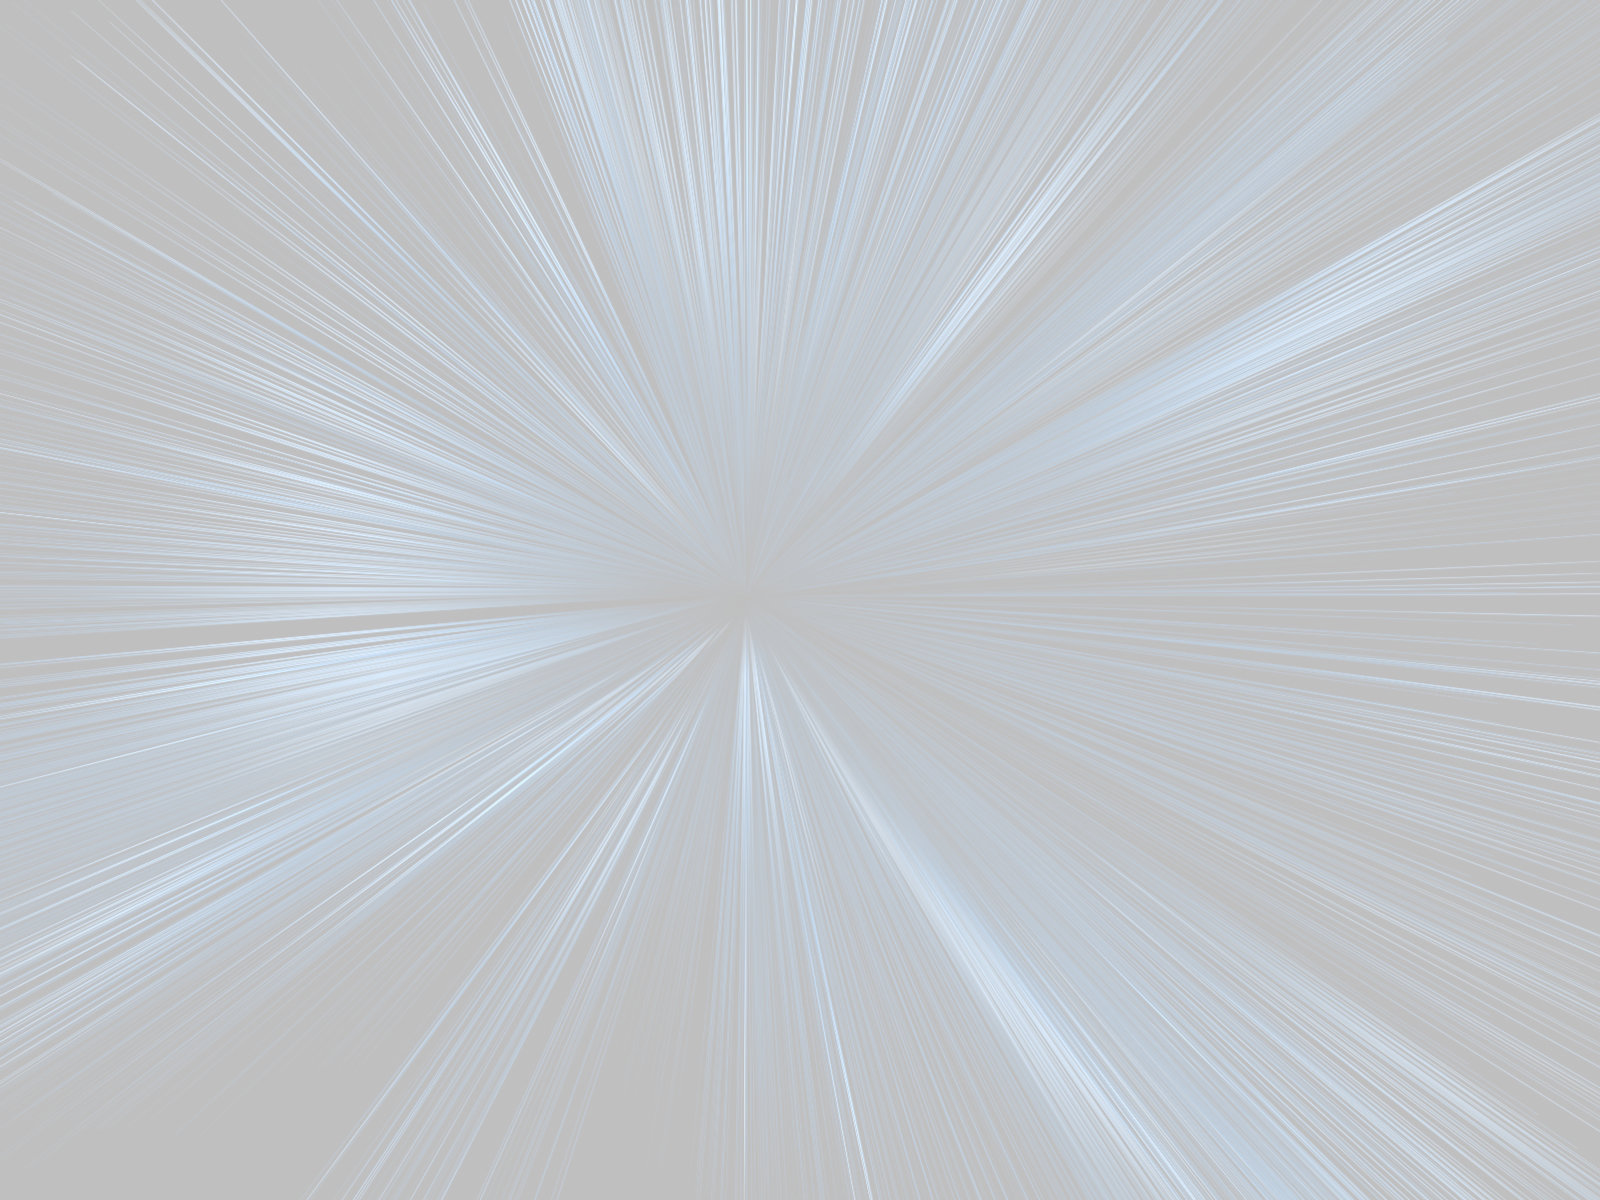
\includegraphics[width=\paperwidth,height=\paperheight]{images/light-speed}
} 

 \addtobeamertemplate{block begin}{\pgfsetfillopacity{0.5}}{\pgfsetfillopacity{1}}
 \addtobeamertemplate{block alerted begin}{\pgfsetfillopacity{0.5}}{\pgfsetfillopacity{1}}
 \addtobeamertemplate{block example begin}{\pgfsetfillopacity{0.5}}{\pgfsetfillopacity{1}}

\setbeamertemplate{navigation symbols}{}

\title{Solve'n Slide}
\subtitle{Game idea pitch}
\author{Hanieh Arjomand-Fard\\Kevin Sawischa\\Markus Ansorge\\Stefan Aicher}
\date{2. May 2017}

\begin{document}
	\maketitle
	%\frame{\tableofcontents[currentsection]}
	
	%\section{Abschnitt 1}
	\begin{frame}
		\frametitle{At a glance}
		\begin{itemize}
			\setlength\itemsep{1em}
			\item Two phases
			\begin{itemize}
				\item Manipulation
				\begin{itemize}
					\item Deform terrain
					\item Place helpers
				\end{itemize}
			\end{itemize}
			\begin{itemize}
				\item Action
				\begin{itemize}
					\item Slope of hills influence your speed
					\item Correct speed leads you to your goal
				\end{itemize}
			\end{itemize}
			\item Each surface has its own friction
			\item special equipment
			\item special movement
		\end{itemize}
	\end{frame}
	
	\begin{frame}
		\frametitle{Big Idea Bullseye}
		\begin{figure}
			\centering
			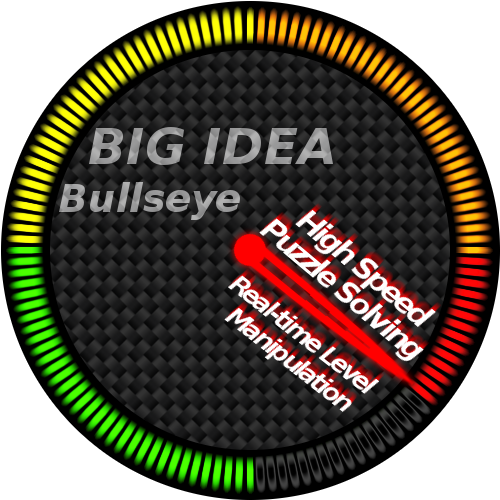
\includegraphics[scale=.4]{images/bigIdeaBullseye}
		\end{figure}
	\end{frame}
	
	\begin{frame}
		\frametitle{Manipulation-Phase}
		\begin{itemize}
			%\setlength\itemsep{1.5em}
			\item Top-down view or free camera movement
			\item Goal not reachable offhand
			\item Raise or lower parts of terrain
			\item Think strategically
			\item Place helpers
			\begin{itemize}
				\item Fuel tanks
				\item Explosives
			\end{itemize}
			\item Limited possibilities to deform
		\end{itemize}
		\begin{figure}[ht]
			\centering
			\begin{tabular}{ccccc}
				\subfloat{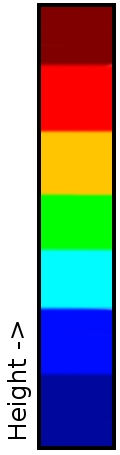
\includegraphics[scale=0.2]{images/HeightScale}}&
				\subfloat{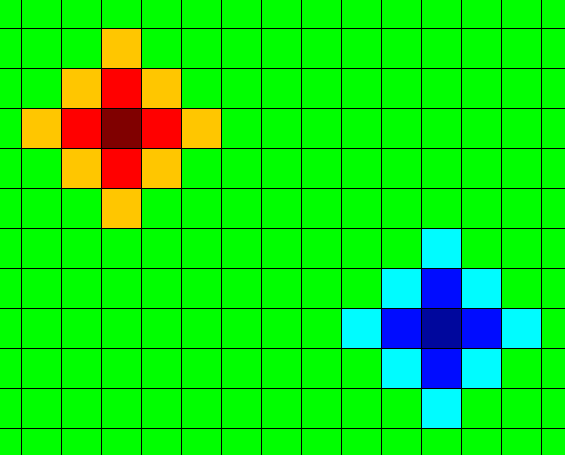
\includegraphics[scale=0.15]{images/Part1IncreaseAndDecreaseCharges}}&
				\subfloat{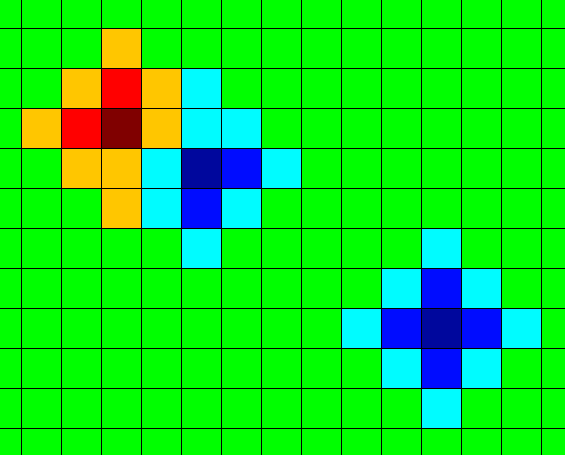
\includegraphics[scale=0.15]{images/Part2DecreaseCharge}}&
				\subfloat{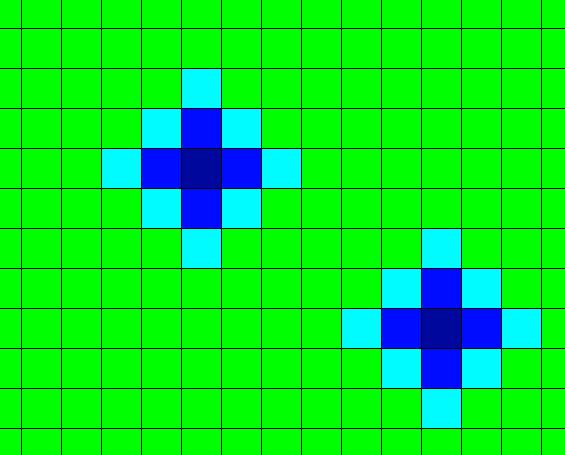
\includegraphics[scale=0.15]{images/Part3RemoveFirstCharge}}
			\end{tabular}
		\end{figure}
	\end{frame}
	
	\begin{frame}
		\frametitle{Technical Achievement}
		\begin{itemize}
			\setlength\itemsep{1.5em}
			\item Real time terrain manipulation different colors
			\item Update terrain geometry and respective textures
			\item Very few parameters make manipulation easy for player
			\item Precise sliding and movement physics depending on slopes
		\end{itemize}
	\end{frame}
	
	\begin{frame}
		\frametitle{Terrain}
		\begin{itemize}
			\setlength\itemsep{1.5em}
			\item Deformable and non-deformable areas are highlighted in different colors
			\item Several landscapes (e.g. grass hills, desert, mountains)
			\item Different surfaces
			\begin{itemize}
				\item Ice $\rightarrow$ no friction
				\item Grass $\rightarrow$ low friction
				\item Pebbles $\rightarrow$ high friction
			\end{itemize}
		\end{itemize}
	\end{frame}
	
	\begin{frame}
		\frametitle{Action-Phase}
		\begin{itemize}
			%\setlength\itemsep{1.5em}
			\item Switch between ego and third-person view
			\item Move along self created hills or walls/ramps
			\item Slopes determine speed/momentum
			\item Use jetpack strategically
			\item Consider friction of different surfaces
		\end{itemize}
		\begin{figure}[ht]
			\centering
			\begin{tabular}{cccc}
				\subfloat{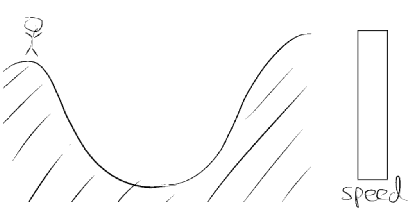
\includegraphics[scale=0.26]{images/StoryboardMovementPart1}}&
				\subfloat{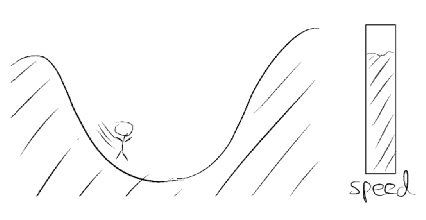
\includegraphics[scale=0.26]{images/StoryboardMovementPart2}}
			\end{tabular}
		\end{figure}
		\begin{figure}[ht]
			\centering
			\begin{tabular}{cccc}
				\subfloat{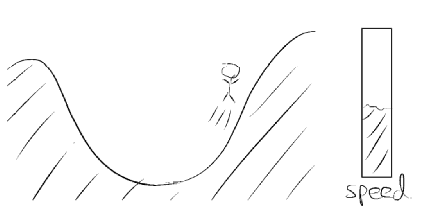
\includegraphics[scale=0.26]{images/StoryboardMovementPart3}}&
				\subfloat{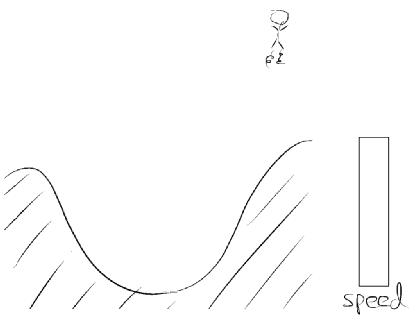
\includegraphics[scale=0.26]{images/StoryboardMovementPart4}}
			\end{tabular}
		\end{figure}
	\end{frame}
	
	\begin{frame}
		\frametitle{Helpers}
		\begin{itemize}
			\setlength\itemsep{1.5em}
			\item Different situations demand different helpers
			\item Grappling hook
			\item Refuel tanks
			\item Wallrunning/magnetic boots
			\item And more
		\end{itemize}
	\end{frame}
	
	\begin{frame}
		\frametitle{Basic Level Example}
		\visible<1,2> {
			\begin{figure}
				\centering
				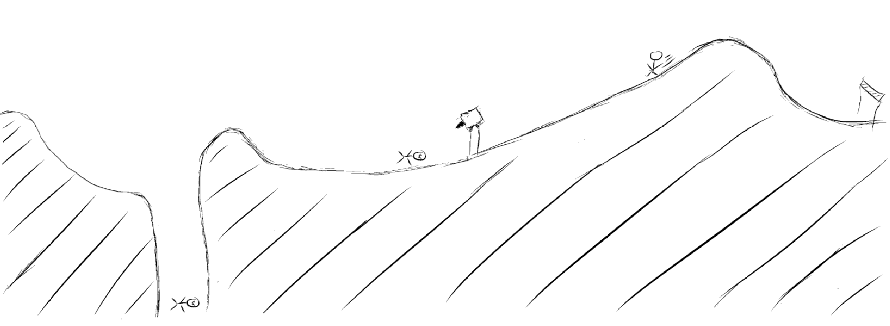
\includegraphics[scale=0.4]{images/LevelWithoutManipulation}
			\end{figure}
		}
		\visible<2> {
			\begin{figure}
				\centering
				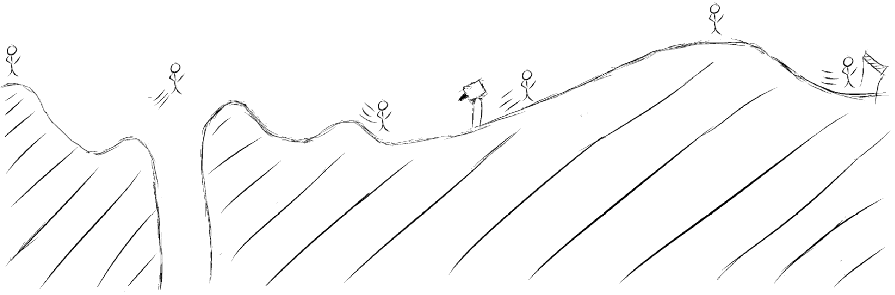
\includegraphics[scale=0.4]{images/LevelWithManipulation}
			\end{figure}
		}
	\end{frame}
	
	\begin{frame}
		\frametitle{The End}
		\centering
		\Huge
		Thanks for your attention.
	\end{frame}
	
	\begin{frame}
		\frametitle{Development Schedule}
		\begin{figure}
			\centering
			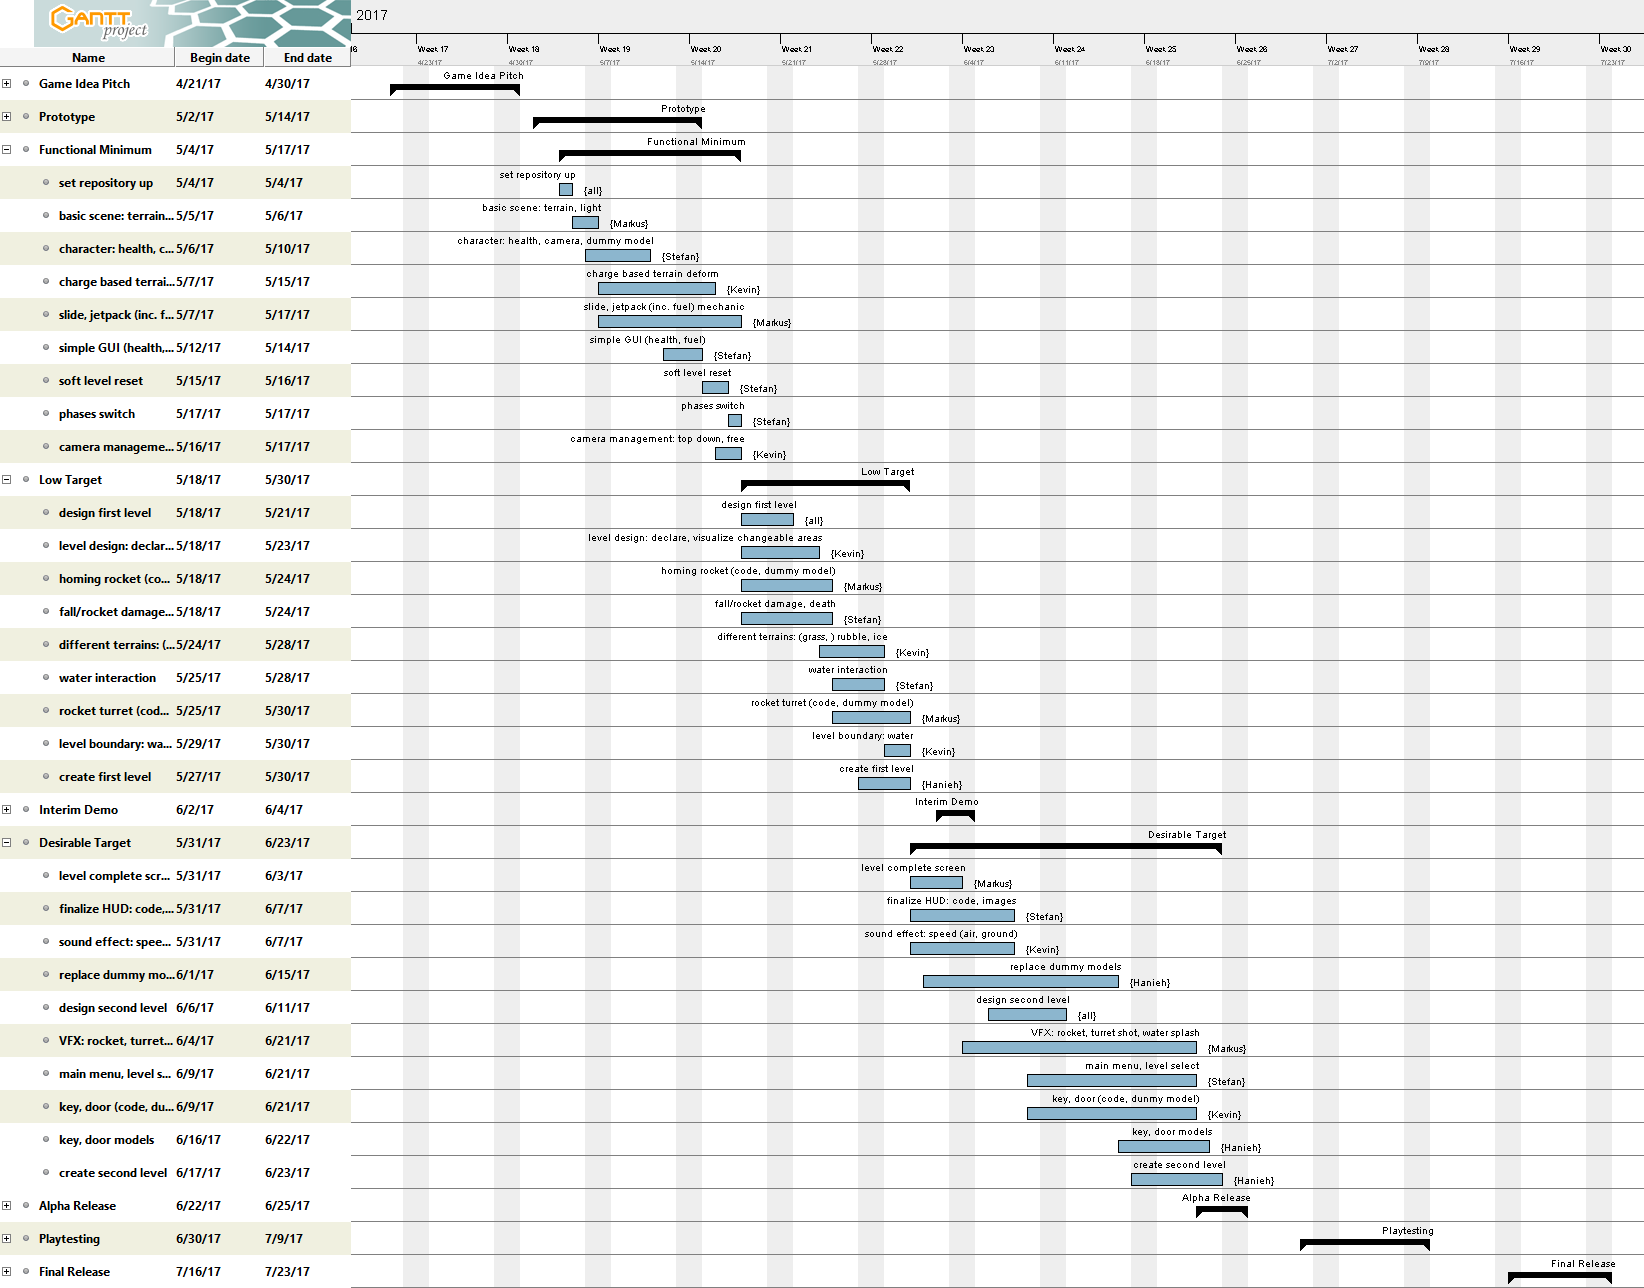
\includegraphics[scale=0.225]{images/GamesLab2017SS_ShortNew}
		\end{figure}
	\end{frame}
\end{document}